\documentclass[conference]{IEEEtran}
\usepackage{amsmath}
\usepackage{amssymb}
\usepackage{graphicx}
\usepackage{booktabs}
\usepackage{cite}
\usepackage{subcaption}
\usepackage{etoolbox}

\graphicspath{{out_dir/}}

\makeatletter
\renewenvironment{abstract}{%
  \normalfont\small\noindent\textbf{Abstract: }\itshape\ignorespaces%
}{%
  \normalfont\par%
}
\makeatother

\begin{document}

\title{PCA-Based Ancestry Analysis Using SNP Data}

\author{
  \IEEEauthorblockN{Yusuf Oguz}
  \IEEEauthorblockA{
    Department of Artificial Intelligence and Data Engineering\\
    Istanbul Technical University\\
    Istanbul, Turkey\\
    150220322
  }
}

\maketitle

\begin{abstract}
In this project, we applied Principal Component Analyis (PCA) and K Nearest Neighbors (KNN) to analiyze human genetic ancestry using Single Nucleotide Polymorphism(SNP) data. The dataset consists of 256 training and 64 test individual from four ancestral populations: Han Chinese in Beijing (CHB), Japanese in Tokyo (JPT), Toscans in Italy (TSI), and Yoruba in Nigeria (YRI).SVD was implemented from scratch using QR iteration with GramSchmidt orthogonalization without relying on any builtin decomposition solvers. PCA correlated SNP scoring was used to reduce the feature space from 5000 SNPs to compact panels. A KNN classifier with $k{=}5$ applied on the top-20 SNP panel achieved 73.44\% test accuracy. TSI and YRI populations were almost perfectly classified while CHB and JPT caused most of the erors which is biologically expected due to their shared East Asian genetic background.
\end{abstract}

\section{Introduction}

Single Nucleotide Polymorphisms (SNPs) are the most common form of genetic variation in humans Each SNP represents a difference at a single position in the DNA encoded as 0, 1, or 2 depending on the number of alternate aleles at that locus. Althought 99.9\% of human DNA is identical across individuals the remaining variation includes SNPs whose frequencies differ significantly between geographic populations These differences make it possible to identify ancestral backgrounds from genetic data alone.

In this project we followed the methodology of Paschou et al \cite{paschou2007}, which proposes using PCA to find a small subset of SNPs that captures the most population relevant variation. The core idea is to score each SNP by its correlation with the top principal components and then use only the highest scoring ones for downstream classification.

We implement the entire numerical pipeline from scratch: SVD via QR iteration (without \texttt{np.linalg.svd} or \texttt{np.linalg.eig}), SNP scoring from PCA loadings, and KNN based ancestry prediction. The goal was to demonstrate that a compact SNP panel can recover population structure almost as well as using all 5000 SNPs.

\section{Methods}

\subsection{Data and Preprocessing}

The training set has 256 indivduals and 5000 SNPs. The test set has 64 individuals(16 per population). Both sets cover four populations: CHB, JPT, TSI, and YRI, drawn from the HapMap3 project \cite{hapmap3}.

Preprocessing was done in the following order. First, SNPs with more than 5\% missing values were remove, and then individuals with more than 10\% missing values were removed. After this filtering step, no samples or SNPs were actually dropped from our dataset, meaning the raw data was already clean enought. Remaining missing values were filled with per SNP column means. Finally the matrix was centered by subtracting the mean of each colum.

For the test set, imputation and centering were applied using the statistics computed from the training set not the test set itself. This is important to prevent data leakage.

\subsection{PCA via SVD (from scratch)}

PCA was performed on the centered trainingmatrix $\mathbf{X}_c \in \mathbb{R}^{N \times M}$ where $N = 256$ and $M = 5000$.

Since $N \ll M$, computing the full $M \times M$ covariance matrix is not practical. Instead we used the $N \times N$ covariance matrix:

\begin{equation}
\mathbf{C} = \frac{1}{N-1} \mathbf{X}_c \mathbf{X}_c^\top
\end{equation}

Egenvalues and eigenvectors of $\mathbf{C}$ were computed using the QR iteration algorithm. Starting from $\mathbf{A}_0 = \mathbf{C}$, each iteration performs a QR decomposition:

\begin{equation}
\mathbf{A}_k = \mathbf{Q}_k \mathbf{R}_k, \quad \mathbf{A}_{k+1} = \mathbf{R}_k \mathbf{Q}_k
\end{equation}

The QR decomposition itself was implemented using modified Gram-Schmidt orthogonalization. The accumulated product of $\mathbf{Q}$ matrices converges to the eigenvector matrix $\mathbf{U}$ of $\mathbf{C}$ and the diagonal of $\mathbf{A}_k$ converges to the eigenvalues. Iterations stop when the sum of below-diagonal absolute values falls below $10^{-8}$ (max 500 iterations).

The right singular vectors $\mathbf{V}$ were then recovered from $\mathbf{U}$ using:

\begin{equation}
\mathbf{v}_k = \frac{\mathbf{X}_c^\top \mathbf{u}_k}{\sigma_k}, \quad \sigma_k = \sqrt{\lambda_k \cdot (N-1)}
\end{equation}

\subsection{SNP Scoring and Panel Selection}

Each SNP was scored by summing the squared loadings across the top $k{=}3$ principal components:

\begin{equation}
\text{score}_j = \sum_{i=1}^{k} V_{ji}^2
\end{equation}

SNPs were then ranked by this score, and panels of size 10, 20, 100, and 200 were selected for comparison. Using $k{=}3$ instead of 2 ensures that SNPs contributing to the third direction of variation are also considered during selection, even though final classification only uses 2 PCs. This approach identifies snps that are most correlated with the directions of maximum genetic variation.

\subsection{KNN Ancestry Prediction}

The test set was projected into the PCA space built from the top20 training SNPs. KNN with $k{=}5$ was used for clasification using euclidean distance in 2D PCA space (PC1 and PC2). Majority voting was applied with ties broken by choosing the class of the closest neighbor.

\section{Results}

\subsection{Eigenvalue Analysis}

\begin{figure}[t]
  \centering
  \begin{subfigure}[b]{0.48\linewidth}
    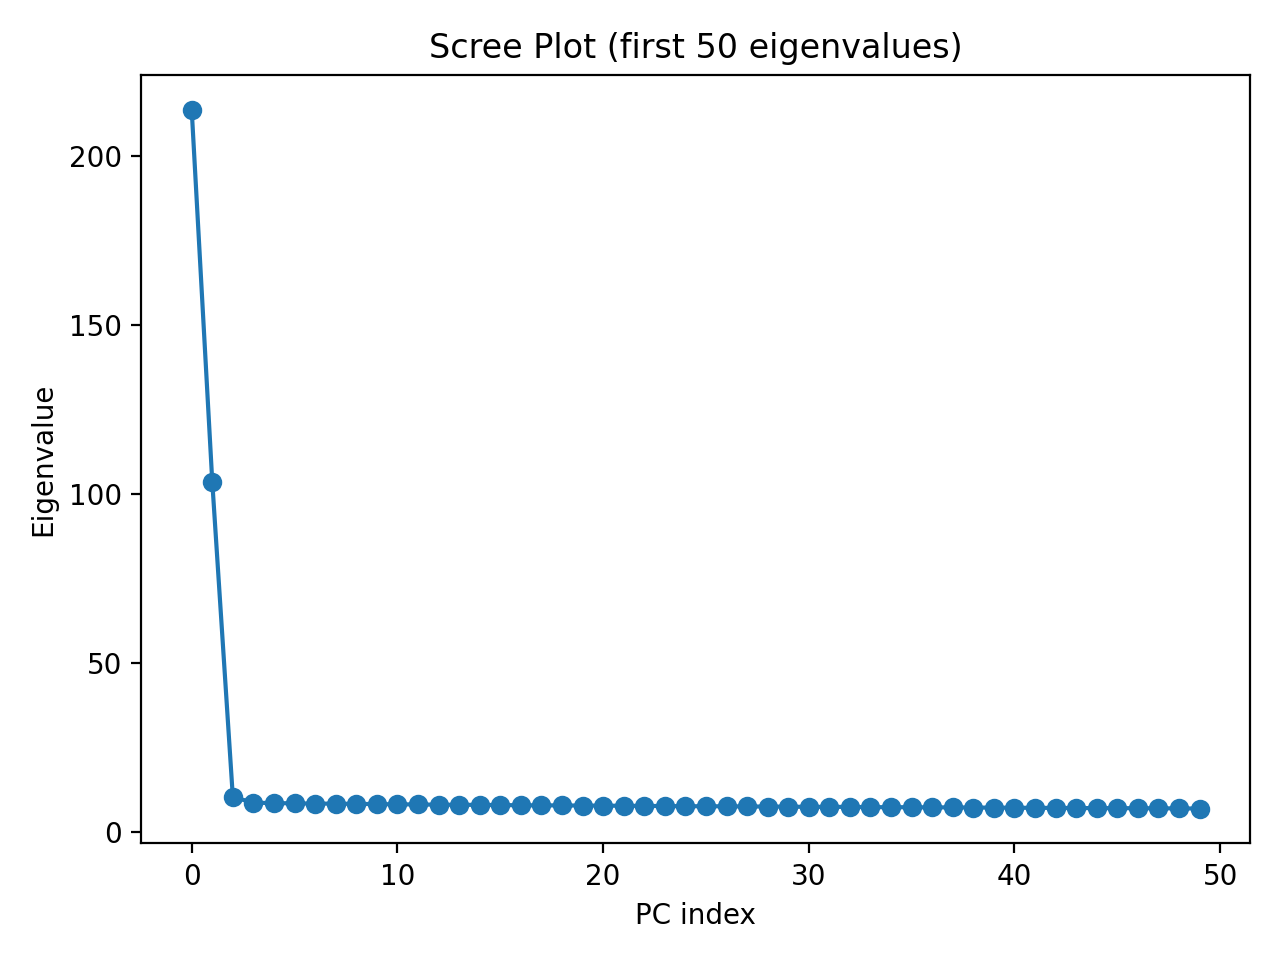
\includegraphics[width=\linewidth]{eigenvalues.png}
    \caption{Scree plot}
  \end{subfigure}
  \hfill
  \begin{subfigure}[b]{0.48\linewidth}
    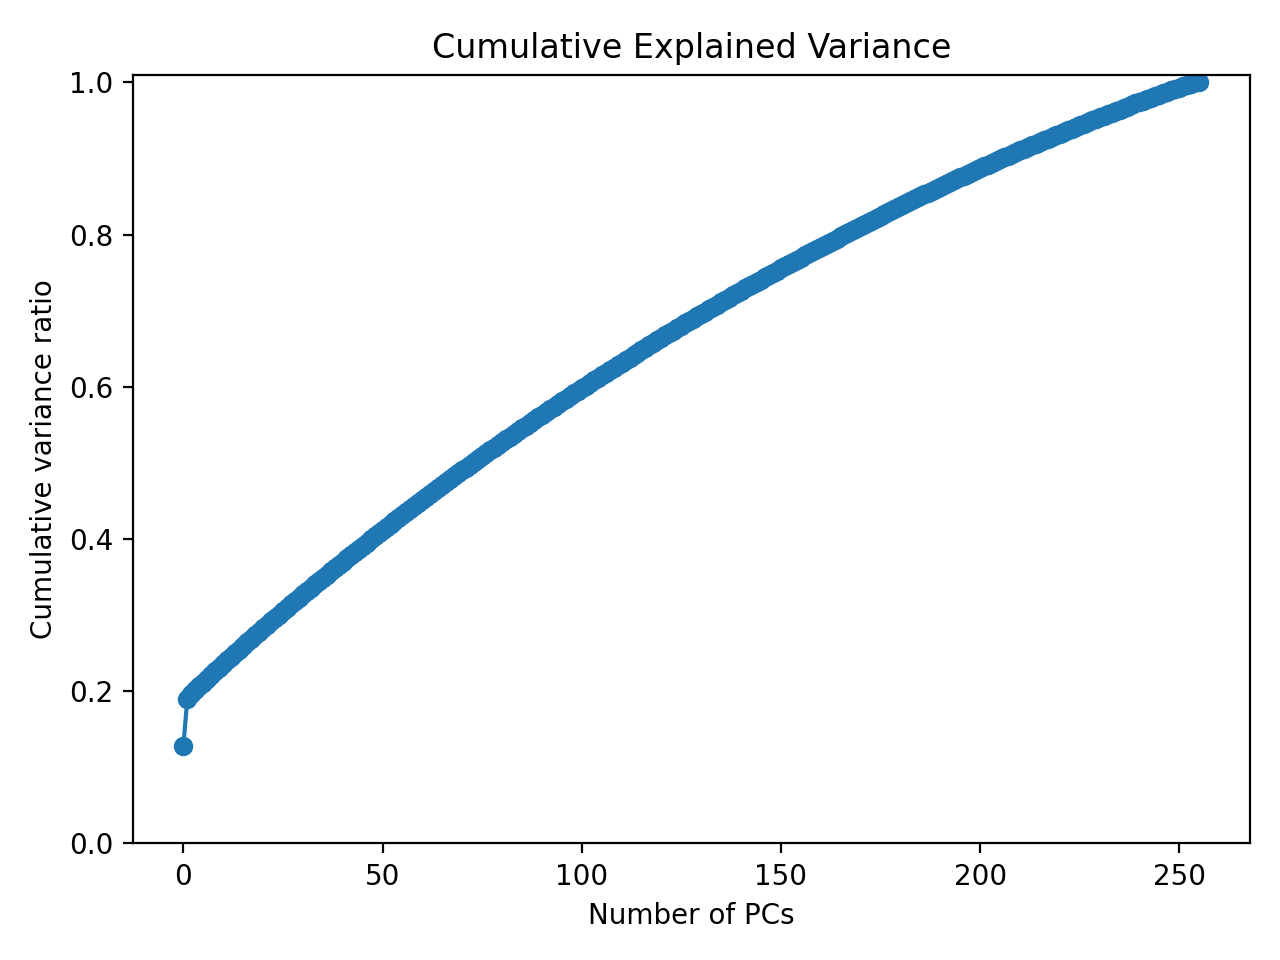
\includegraphics[width=\linewidth]{cumulative_variance.png}
    \caption{Cumulative variance}
  \end{subfigure}
  \caption{Eigenvalue analysis of the full 5000-SNP PCA.}
  \label{fig:eigen}
\end{figure}

The first two PCs explain 12.80\% and 6.20\% of total variance respectively giving a cumulative 18.99\%. Although this number looks small it is actually typical for SNP data because most SNPs vary independently and the genetic signal is spread across many loci. The scree plot shows a clear elbow after the first two component which indicates that PC1 and PC2 carry the most population structure information.

\subsection{Population Structure Visualization}

\begin{figure}[t]
  \centering
  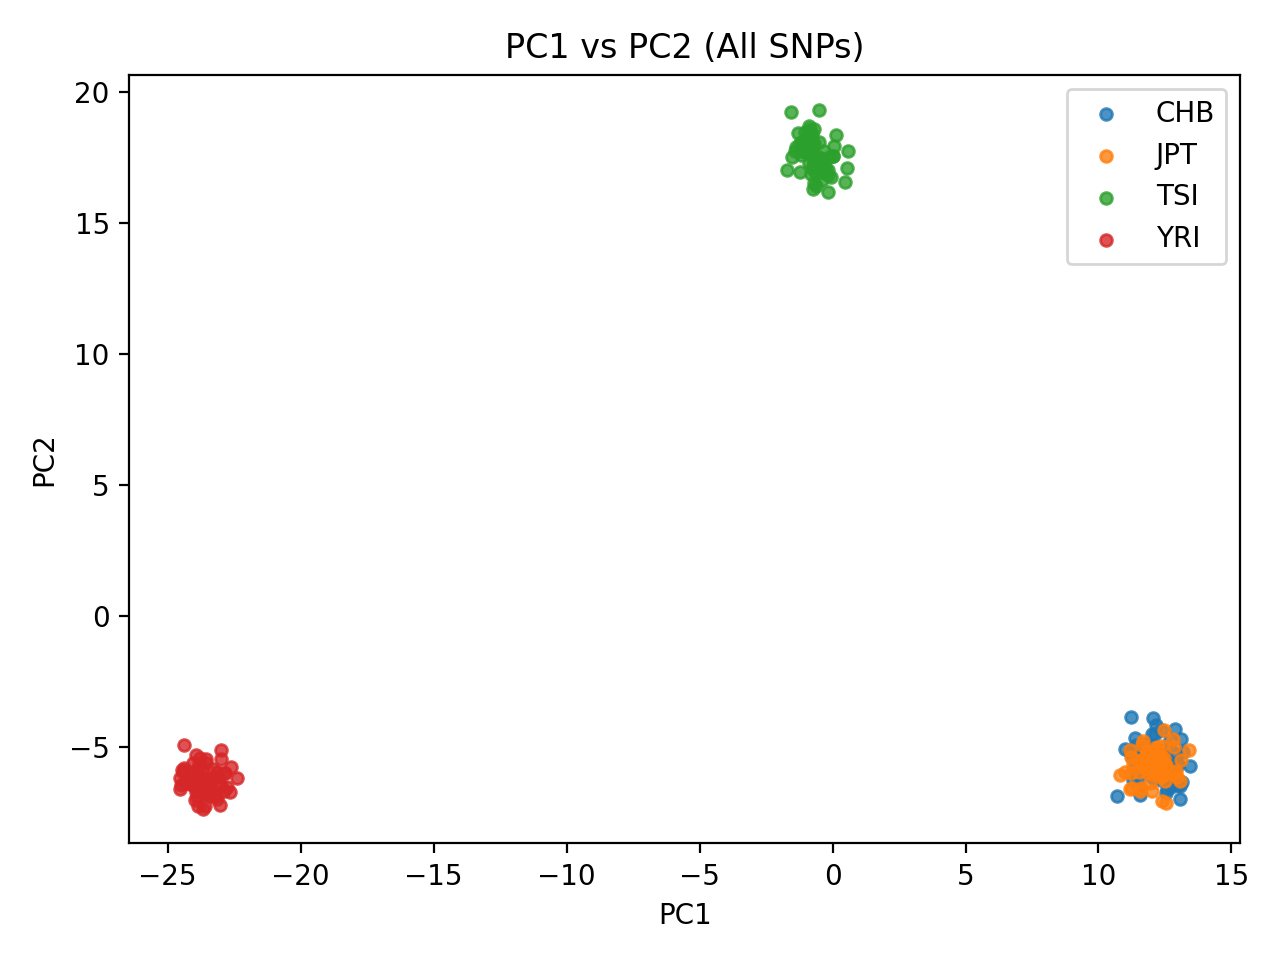
\includegraphics[width=0.9\linewidth]{pc_scatter_all_snps.png}
  \caption{PC1 vs PC2 scatter plot using all 5000 SNPs. Training individuals are colored by population.}
  \label{fig:scatter_all}
\end{figure}

The PC scatter plot using all 5000 SNPs shows that the four populations form visible clusters. YRI (African) is clearly separated from the other three populations along PC1. TSI (European) forms a distinct cluster along PC2. CHB and JPT both fall in a similar region which shows that they have very close genetic profiles. This is expected since they are both East Asian populatons.

\subsection{Effect of SNP Panel Size}

\begin{figure}[t]
  \centering
  \begin{subfigure}[b]{0.48\linewidth}
    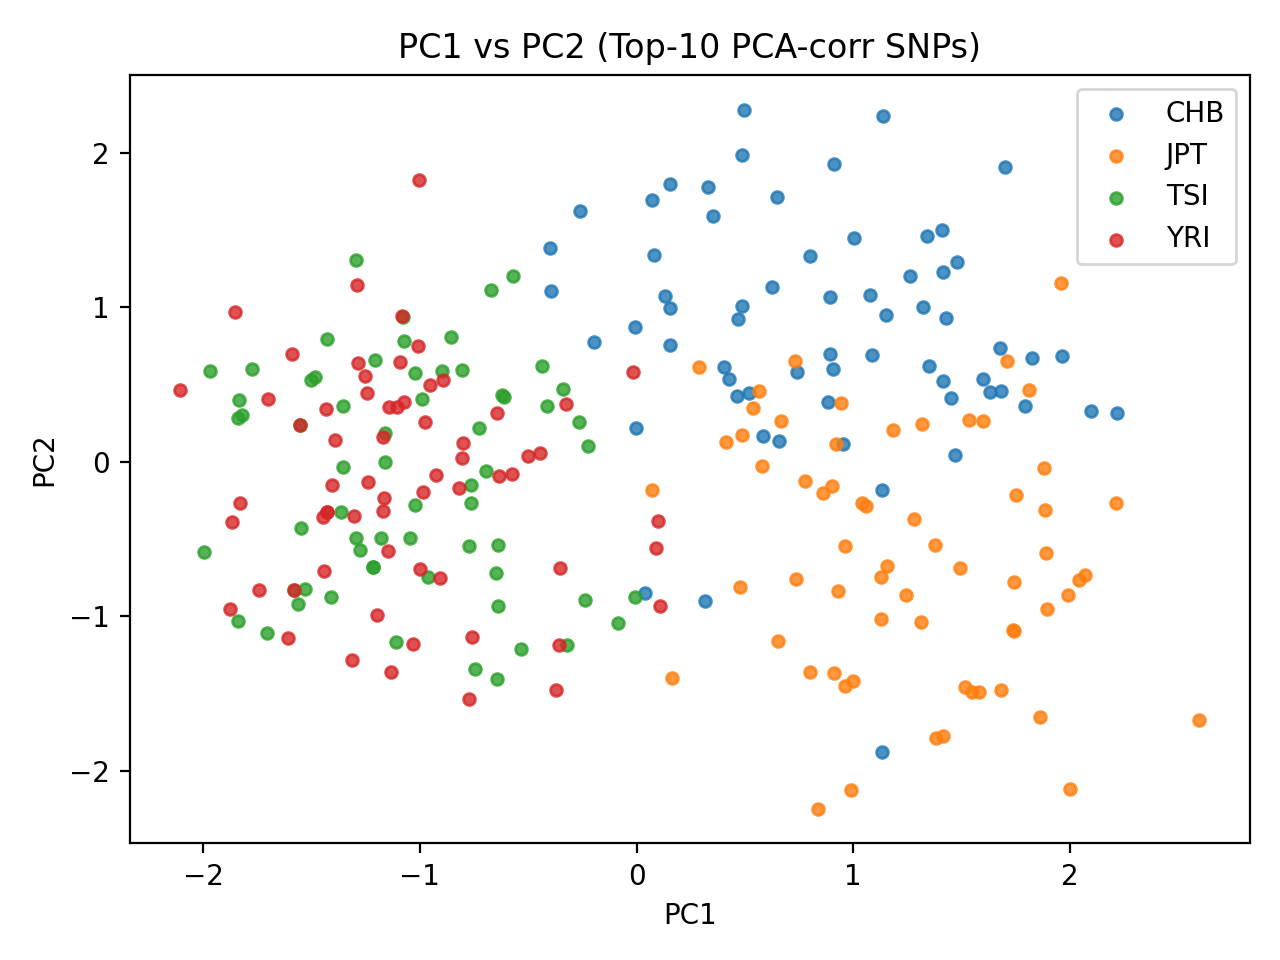
\includegraphics[width=\linewidth]{pc_scatter_top_10.png}
    \caption{Top-10 SNPs}
  \end{subfigure}
  \hfill
  \begin{subfigure}[b]{0.48\linewidth}
    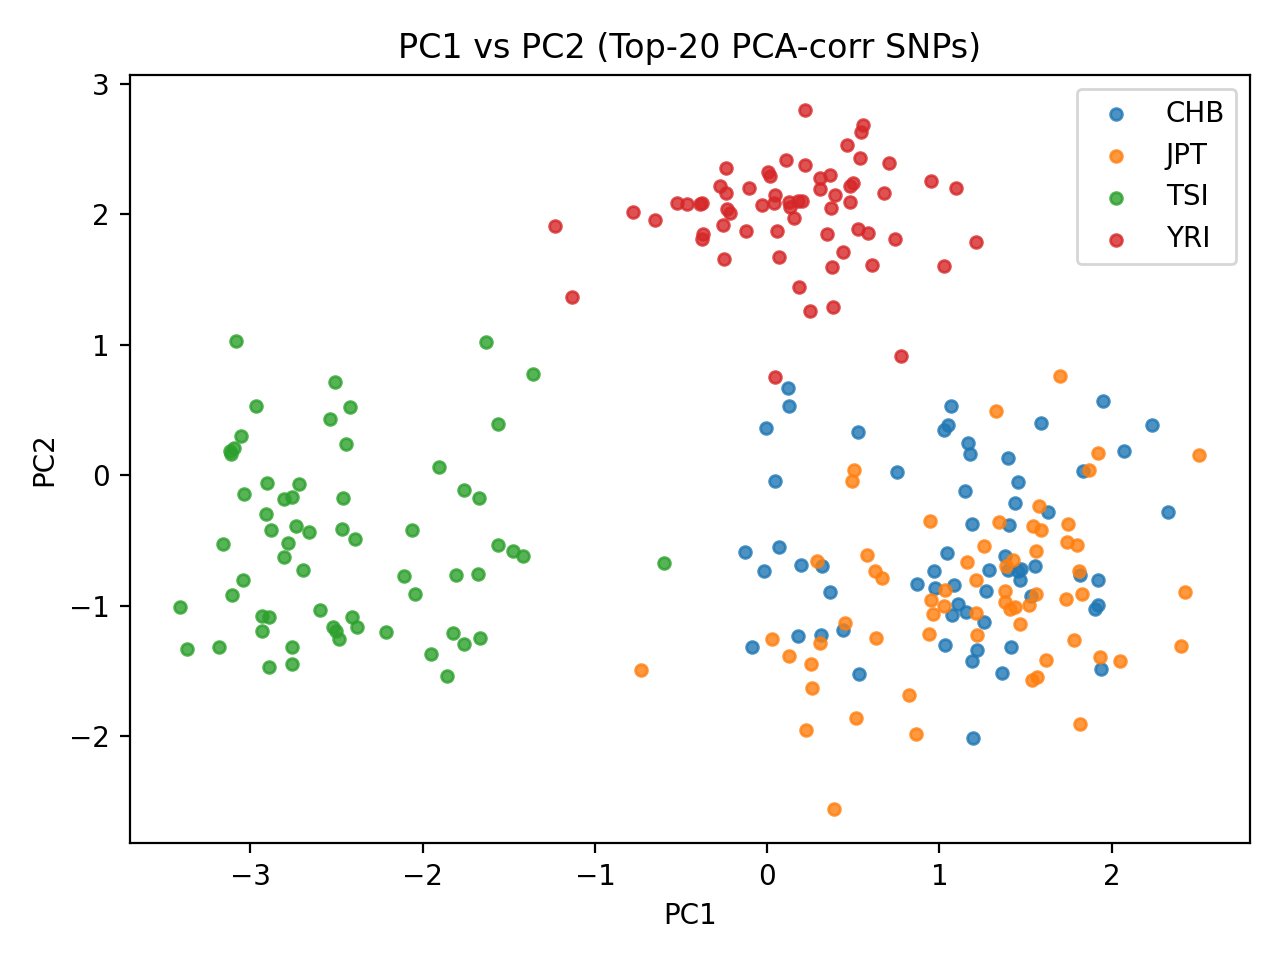
\includegraphics[width=\linewidth]{pc_scatter_top_20.png}
    \caption{Top-20 SNPs}
  \end{subfigure}

  \vspace{2pt}
  \begin{subfigure}[b]{0.48\linewidth}
    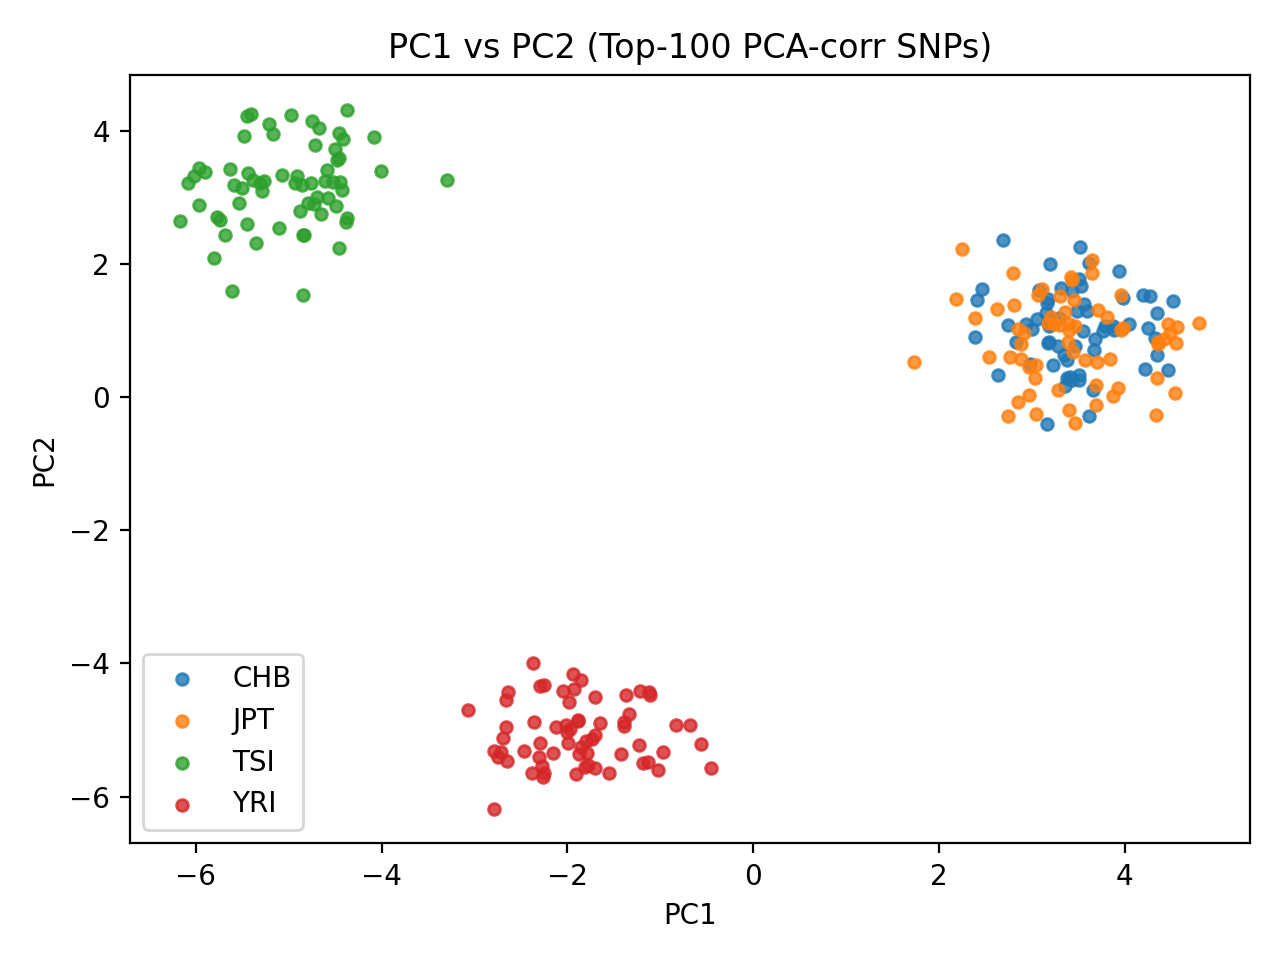
\includegraphics[width=\linewidth]{pc_scatter_top_100.png}
    \caption{Top-100 SNPs}
  \end{subfigure}
  \hfill
  \begin{subfigure}[b]{0.48\linewidth}
    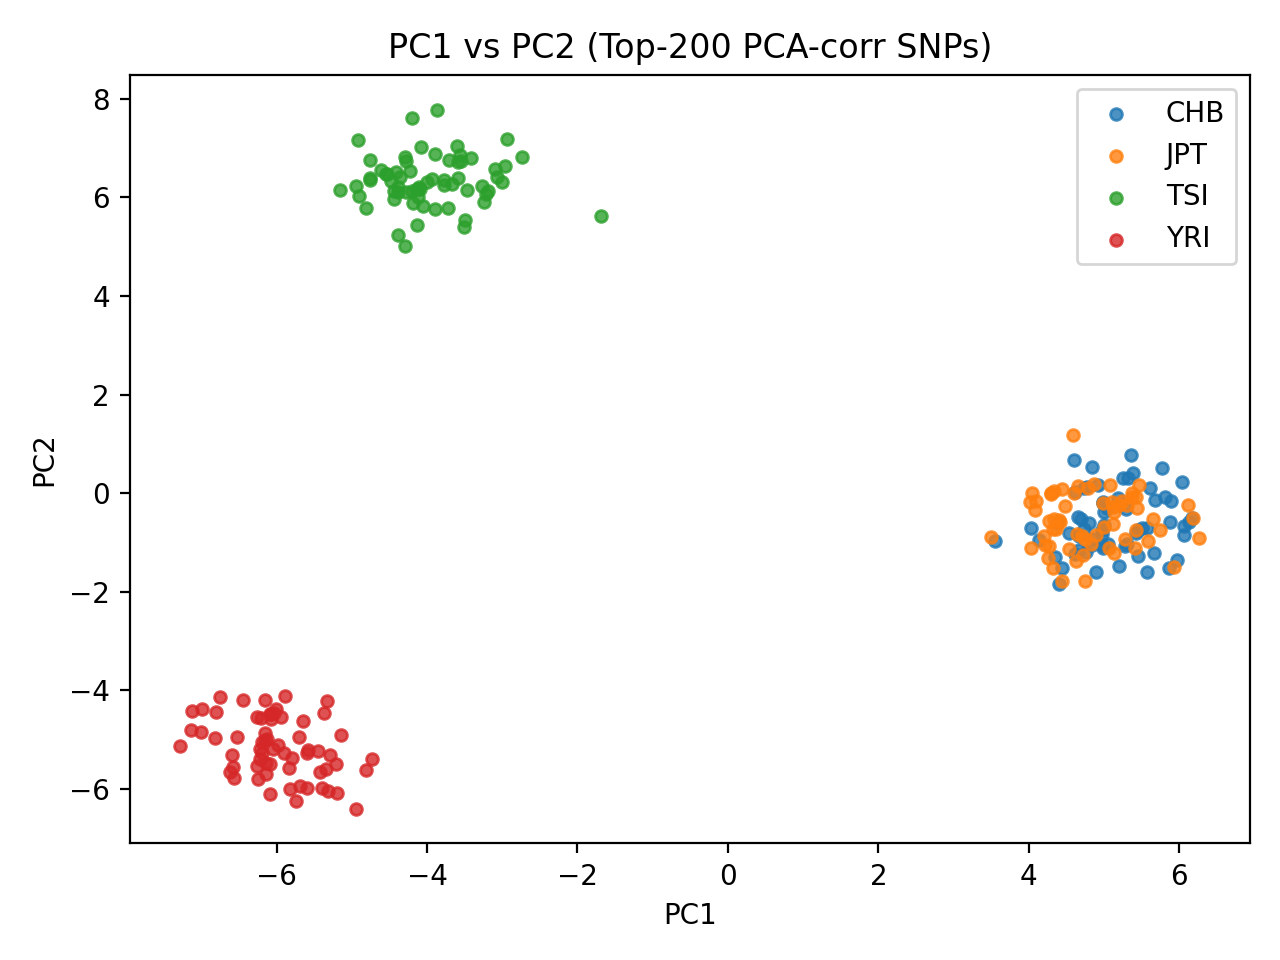
\includegraphics[width=\linewidth]{pc_scatter_top_200.png}
    \caption{Top-200 SNPs}
  \end{subfigure}
  \caption{PC scatter plots for different SNP panel sizes.}
  \label{fig:panels}
\end{figure}

Even with only 10 SNPs, the four populations are mostly separated. The top-20 panel already provides cluster separation that is visually comparable to the full 5000-SNP result. Increasing the panel to 100 or 200 SNPs gives slightly cleaner separation but the improvement is not dramatic. This shows that the PCA correlated scoring method is effective at finding a compact and informative subset.

\subsection{Ancestry Prediction Performance}

\begin{figure}[t]
  \centering
  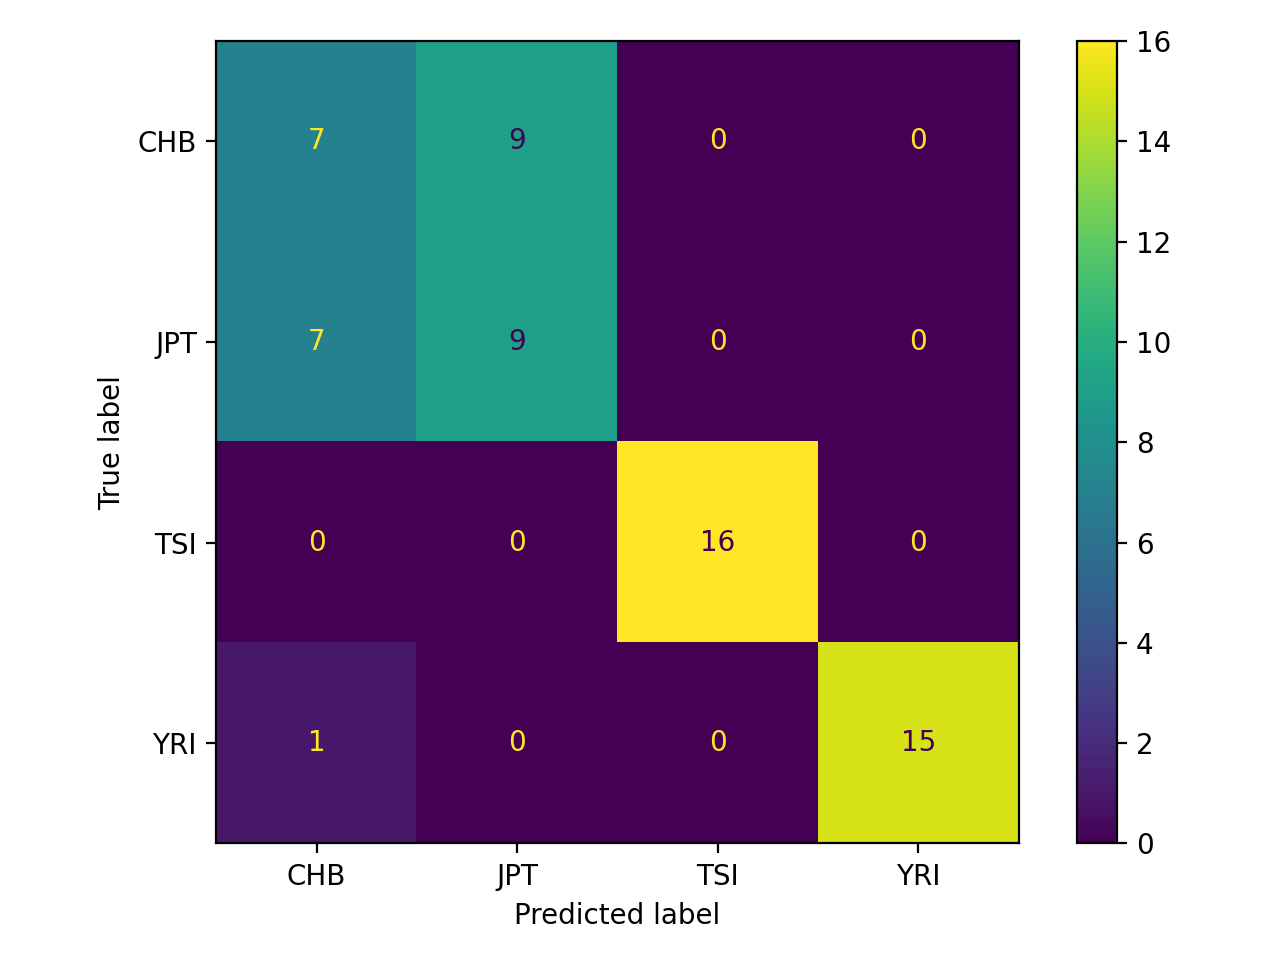
\includegraphics[width=0.75\linewidth]{confusion_matrix.png}
  \caption{Confusion matrix for KNN ($k{=}5$) on the test set using top-20 SNPs.}
  \label{fig:cm}
\end{figure}

The overall test accuracy was \textbf{73.44\%} (47 out of 64 correct). Table \ref{tab:acc} summarizes per-population results. TSI and YRI are almost perfectly classified. The main source of errors is the CHB/JPT pair: most CHB individuals are predicted as JPT and vice versawhich reflects the significant genetic overlap between these two populations.

\begin{table}[h]
  \centering
  \caption{Per-population classification accuracy (test set).}
  \label{tab:acc}
  \begin{tabular}{lcc}
    \toprule
    Population & Correct / Total & Accuracy \\
    \midrule
    CHB & 7 / 16 & 43.75\% \\
    JPT & 9 / 16 & 56.25\% \\
    TSI & 16 / 16 & 100.00\% \\
    YRI & 15 / 16 & 93.75\% \\
    \midrule
    Overall & 47 / 64 & 73.44\% \\
    \bottomrule
  \end{tabular}
\end{table}

\section{Discussion}

The results show that the PCA-correlated SNP scoring approach works well for identifying ancestry-informative markers. Using only 20 SNPs out of 5000 (0.4\% of the original features) we can achieve reasonable classification performance for most populations.

The biggest  limitation is the CHB/JPT confusion. These two populations are geographically close and have been exchanging genes throughout history, so they are much harder to distinguish genetically compared to continental level differences like East Asian vs European or African. In 2d PCA space, their clusters strongly overlap, so KNN can not reliably separate them with just 20 SNPs.

One possible improvement would be to classify in a higher dimensional PCA space, e.g. using PC1, PC2 and PC3 together instead of just 2 PCs. The cumulative variance plot suggests that PC3 might carry some additional discriminating information specifically for the CHB/JPT pair, which is not captured in the 2D projection.

Another thing worth mentioning is the QR iteration convergence. For this dataset, the covariance matrix eigenvalues are wel separated (PC1 eigenvalue is about twice PC2, which is about 10 times PC3), so the QR algorithms converged quickly and gave stable result.

\section{Conclusion}

In this project we built a complete pipeline for SNP based ancestry analysis using only basic matrix operations. SVD was implemented via QR iteration with Gram-Schmidt orthogonalization. The PCA correlated SNP scoring method successfully identified informative markers and reduced the feature space by 250x. KNN in the reduced PCA space achieves good performance for TSI and YRI population but struggle with CHB/JPT, which is consistent with their genetic similarity. Overal the result confirm the effectiveness of the Paschou et al. method for population structure analysis.

\begin{thebibliography}{9}

\bibitem{paschou2007}
P. Paschou, E. Ziv, E. G. Burchard, S. Choudhry, W. Rodriguez-Cintron, M. W. Mahoney, and P. Drineas,
``PCA-correlated SNPs for structure identification in worldwide human populations,''
\textit{PLoS Genetics}, vol. 3, no. 9, p. e160, 2007.

\bibitem{hapmap3}
The International HapMap 3 Consortium,
``Integrating common and rare genetic variation in diverse human populations,''
\textit{Nature}, vol. 467, no. 7311, pp. 52-58, 2010.

\end{thebibliography}

\end{document}
